% vim: set fenc=utf-8 ft=latex encoding=utf-8
% -*- mode: latex; coding: UTF-8; -*-
%!TEX root = knowledge-curation.tex
\section{Methodology}
\label{cha:methodology}

    We carried out a qualitative case study of the knowledge that flows through the channel. 
    This method is considered to be suitable for studies that explore under-researched phenomena and for providing an in-depth analysis within its real-life context~\cite{Yin2009}.

%	This chapter describes the elements of the methodology, including the research questions, the adopted case study methodology, and the phases of the study.
%	This chapter also outlines the procedure used to collect and analyse the data in this study.

%\subsection{Research Questions}

%	The four research questions that guided this thesis are:

%\paragraph*{RQ-1. What types of knowledge are shared on Stack Overflow and the R-help mailing list within the R community?}

%	In the R community, the R-help mailing list serves the same purpose as Stack Overflow.
%	This led to the question of \emph{what types of knowledge are shared on Stack Overflow and the R-help mailing list?}
%	To answer this question I proceeded to analyse and categorize the knowledge in questions, answers, updates, comments and flags on Stack Overflow and the R-help mailing list.
%	Based on the analysis I was able to contrast the way knowledge flows through Stack Overflow and the R-help mailing list.

%\paragraph*{RQ-2. How is the knowledge constructed on Stack Overflow and the R-help mailing list?}

%	As discussed before, Stack Overflow and the R-help mailing list support the R community. 
%	Such a statement implies that the interactions hosted by these two media channels are of a collaborative nature.
%	I wondered if the same applies to the creation and sharing of knowledge in these two channels.
%	My goal was to identify the mechanisms and strategies on Stack Overflow and the R-help mailing list used to construct knowledge collaboratively and individually (if any).

%\paragraph*{RQ-3. How does the sharing of links on Stack Overflow and the R-help mailing list support knowledge construction?}

%	On the Internet, links support the reuse and referencing of data from other resources.
%	Links contain information that is valuable for messages, and depending on how they are used, links can support knowledge sharing practices in different ways.
%	For instance, a link can expand what is known about a topic by referencing more complete sources of information, or provide data to reproduce certain behaviours on source code examples.
%    Previously, I have identified the types of links on Stack Overflow and how they support diffusion of knowledge~\cite{Gomez2013}.
%	For this study, I pursued the identification of how links contribute to the construction of knowledge.
%	Thus, I categorized links posted in the body of messages on Stack Overflow and the R-help mailing list based on their type (e.g., Q\&A Website, and Forums), and how each type of link supported the knowledge construction.

%\paragraph*{RQ-4. Why do certain users post to both Stack Overflow and the R-help mailing list?}

%	As mentioned by Vasilescu~\cite{Vasilescu2014b}, there is a group of users that are active on Stack Overflow and the R-help mailing list. 
%	I wondered if there were any advantages or disadvantages on using both channels.
%	With that in mind, I identified a list of active users in both channels and used open coding methods to analyse their posts.

%\subsection{Case Study Methodology}
%
%	A case study facilitates the exploration of a phenomenon within its context using a variety of data sources~\cite{Yin2009,Yin2012}.
%	In software engineering, a \textit{case study} is defined as  \textit{``an empirical enquiry that draws on multiple sources of evidence to investigate one instance (or a small number of instances) of a contemporary software engineering phenomenon within its real-life context, especially when the boundary between phenomenon and context cannot be clearly specified''}~\cite{Runeson2012}.
%
%	Yin~\cite{Yin2012} states that a case study should be used when: 
%	(1) ``How'' or ``why'' questions are trying to be answered; 
%	(2) the researcher cannot manipulate the behaviours of those involved in the study; 
%	(3) the context is an important part of the study; 
%	(4) there is no clear difference in what is happening between the phenomenon and the context; 
%	and (5) when multiple sources of evidence have to be covered.
%	These conditions apply to the nature of this study and its research questions, and motivated the selection of the case study methodology for this work.
%	Specifically, this work is an exploratory case study to explain the interplay of multiple media channels within a community in terms of the knowledge created and shared.
%	%Our goal is to gain insights and compare the usage of selected media channels within the R community. \remarks{Check if this is the same everywhere}
%
%	The study is divided in two phases that were performed in parallel: mining of data archives, and the survey.
%	Figure \ref{fig:StudyPhases} depicts the general organization of the study design.
%	In the next sections of this chapter, each phase is explained in detail.

%	\begin{figure} [!ht]
%		\centering
%		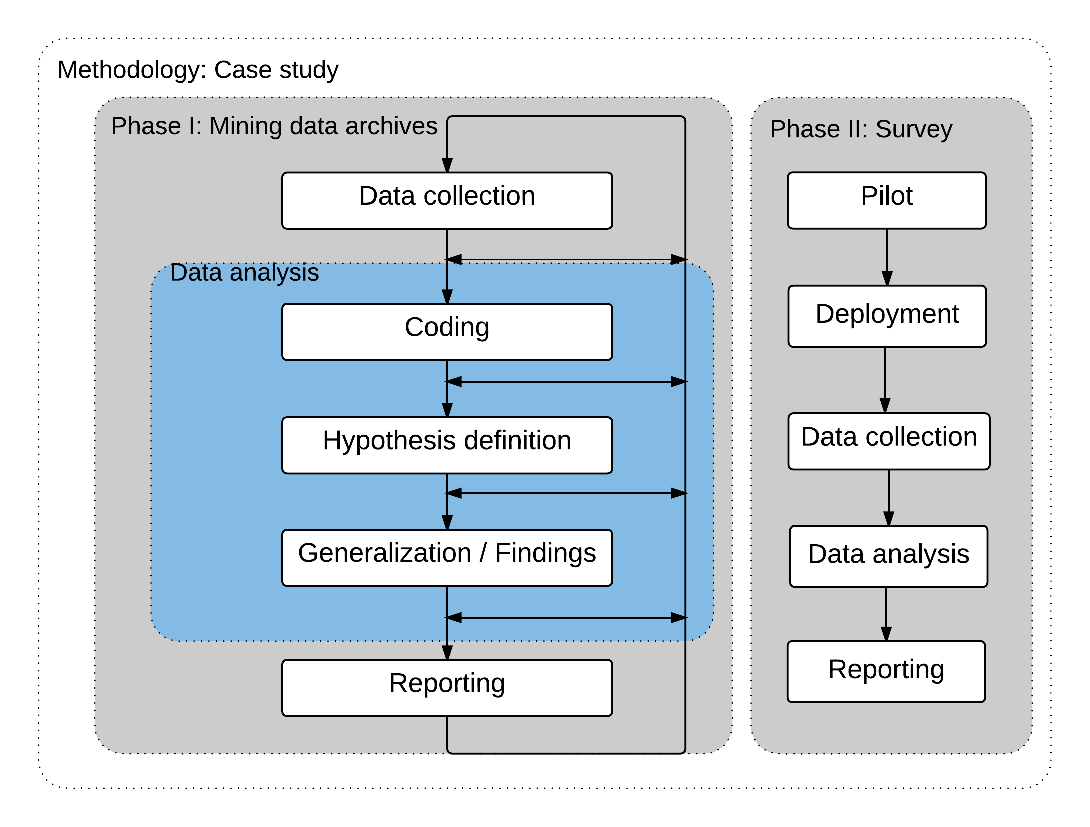
\includegraphics[width=\columnwidth]{Figures/StudyPhases}
%		\caption{General overview of the study design}
%		\label{fig:StudyPhases}
%	\end{figure}

\subsection{Phase 1: Mining data archives} 
\label{sec:studyDesign}

	The mining of the data archives method involved a three step process: data collection, data analysis, and reporting.%~\cite{Runeson2012}.
	The \textbf{data collection} step consisted in gathering the body of data required for analysis.
	This data was a selected set of R-related posts from Stack Overflow and the R-help mailing list.
	In the \textbf{data analysis} step, we analysed the data by looking for answers for the research questions.
	Finally, the \textbf{report} step, we consolidated the results, which are presented in section~\ref{cha:findings}.

\subsubsection{Data collection and preparation}
\label{subsec:preparation}

	Stack Overflow and the R-help mailing list store their messages in publicly available archives.
	The records available for Stack Overflow start in 2008 (the birth of Stack Overflow), while the R-help archives go back to 1997.
	To make both data sets comparable, we analysed the data from 2008 until 2013, a period of time that both channels were available simoultaneously.
For Stack Overflow, we obtained a data dump file available in its website.
For the R-help mailing list data, we retrieved the archives available as MBOX files from the R website.

	We used two different software tools to prepare the data.
	\begin{enumerate*}[label=(\arabic*)]
	\item to process the Stack Overflow data, we used a modified version of Sam Saffron's application, So-Slow\footnote{\url{https://github.com/SamSaffron/So-Slow}}; and,
	\item to process the R-help mailing list archives, we wrote a software application\footnote{Our tool is available at \url{https://github.com/cagomezt/GTMail}}, based on the Bettenburg \textit{et al}~\cite{Bettenburg2009} recommendations of how to process mailing list data.
	\end{enumerate*}
    Once we pre-processed the data, we stored them in a database for further analysis.

%	The following subsections detail the analysis process for each media channel.

%\subsubsection{The R-help mailing list}
%\label{subsec:r-help}

To ensure accurate results when processing the R-help mailing list, we followed the series of recommendations proposed by Bettenburg \textit{et al}.~\cite{Bettenburg2009}.
To make the data comparable againt the Stack Overflow dat set, we transformed the email addresses to MD5 hashes, and changed the time zone of the mailing list messages (UTC+2) to the time zone used by Stack Overflow (UTC).

%\subsubsection*{Stack Overflow}
Stack Exchange releases a new data dump from all their websites every three months\footnote{\url{http://stackexchange.com/sites}}.
However, the last dump file that containing email addresses as MD5 hashes was released in September 2013.
Since then, Stack Overflow does not provide the email addresses.
Because of this, we used the data dump file from September 2014, but updated the table \texttt{users} with the hashes in the dump file from September 2013, for whose \texttt{ID}s were identical in both data sets.
If an user from the 2013 data file did not exist in the 2014 data, we ignored it.
%	As stated previously, I used a modified version of Sam Saffron's application, So-Slow.
%	The purpose of this is to extract the information in the file using XML tags (e.g., post, user, and comment), and load it in a database.
We filtered all R-related data by selecting only messages with the R tag (\texttt{r}) and its synonyms\footnote{\url{http://stackoverflow.com/tags/r/synonyms}} (\texttt{rstats} and \texttt{r-language}).

	Table~\ref{table:data} depicts a summary of the data uploaded in the database.
	The R-help has more questions, answers, and users than Stack Overflow, because there were approximately ten years of additional data.
	Only Stack Overflow's data contains ``comments'' information. %so this field is empty for the R-help mailing list column.

	\begin{table}[!htb]
	  \centering
      \caption{Raw data collected for each channel.}
      \begin{small}
        \begin{tabular}{lrr}
	        \toprule
	        Type          &  R-help & Stack Overflow \\
	        \midrule
	        Questions     & 101,931 &  67,393 \\
	        Answers       & 213,366 &  99,620 \\
	        Comments      &       - & 286,124 \\
	        Users         &  39,150 &  26,324 \\
	        \bottomrule
        \end{tabular}
      \end{small}
	  \label{table:data}
	\end{table}


%\subsubsection*{Data merging}
%	There are some studies that propose different techniques for merging users' identities by analysing the data from multiple repositories (e.g., mailing lists, bug tracking information, and source code management tools)~\cite{Bird2006, Kouters2012,Vasilescu2014c}.
%	Bird \textit{et al}.~\cite{Bird2006} proposed a heuristic to match users' identities across multiple mailing list archives by combining parts of user names and email addresses. For example, the \textit{cagomezt} prefix is likely to belong to \textit{Carlos Arturo Gomez Teshima}.
%	Furthermore, Kouter \textit{et al}.~\cite{Kouters2012} used a natural language processing technique called Latent Semantic Analysis to merge identities on very noisy data.
%	However, it has been demonstrated that all existing approaches produce false positives and false negatives~\cite{Goeminne2013}.

To merge both datasets, we matched Stack Overflow's email MD5 hashes with the MD5 hash version of email addresses from the R-help mailing list data.
We did not use any method to infer email addresses based on user names.
%In practice, this conservative approach~\cite{Vasilescu2014b}
The resulting set was 1,421 different users with the same email address on both media channels.

%	Because Stack Overflow only provides the email addresses as MD5 hashes, and to make both data sets comparable, the mailing list emails were converted to their corresponding MD5 hashes.

Although MD5 hashes are not \textit{collision resistant} and could possibly lead to false positives, it is unlikely that two different email addresses share a MD5 hash.
%    The probability to find a MD5 collision is less than $1/2^{64}$~\cite{Rivest1992}.
	%\footnote{\url{https://en.wikipedia.org/wiki/Collision_resistance}}, and therefore, this could possibly lead to false positive resistant outcomes.

\subsubsection{Data analysis process}
\label{sec:dap}

To analysis the data that flows through Stack Overflow and the R-help mailing list, we performed a qualitative and exploratory approach, as it best suits research when a concept or phenomenon requires more understanding, with little pre-existing research~\cite{Creswell2009}.

In particular, we performed an inductive approach~\cite{Runeson2012} to analyse the data from Stack Overflow and the R-help mailing list.
This is an iterative process, where across the study is necessary to switch between data selection and data analysis, or between data reporting and data collection.
As advised to reduce bias~\cite{Runeson2012}, two researchers conducted the analysis, both computer scientists with a background in qualitative data analysis.

\begin{figure*}[!htb]
	\centering
	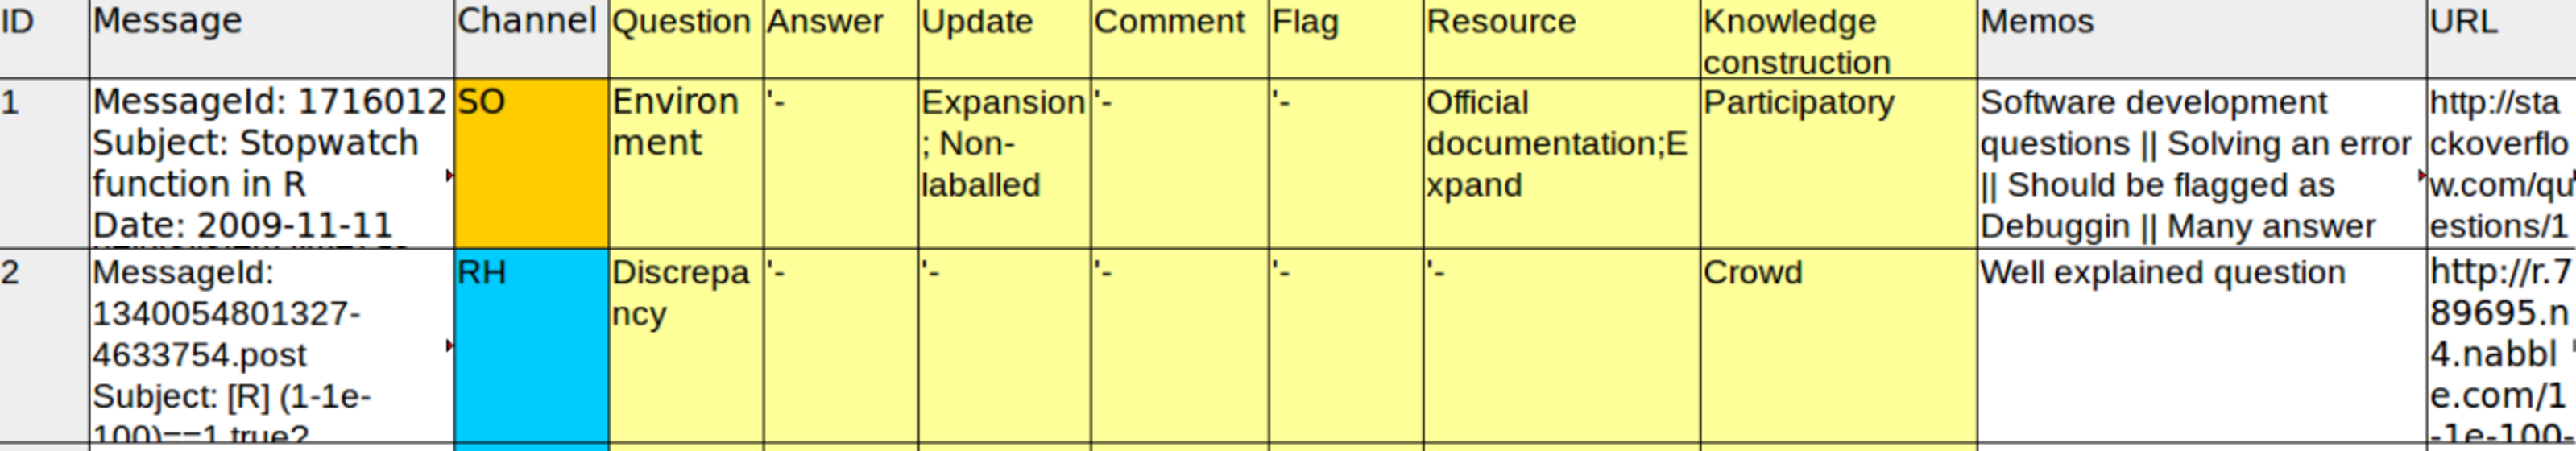
\includegraphics[width=.9\textwidth]{Figures/CodingExample}
	\caption{Example of data coding. Each row is a thread message. Questions, comments, and answers are identified with the number on the first column. Columns in yellow contain the codification for each message type. The last two columns contain the memos and the URL.}
	\label{fig:CodingExample}
\end{figure*}

%	%<<
%	\begin{figure} [!htb]
%		\centering
%		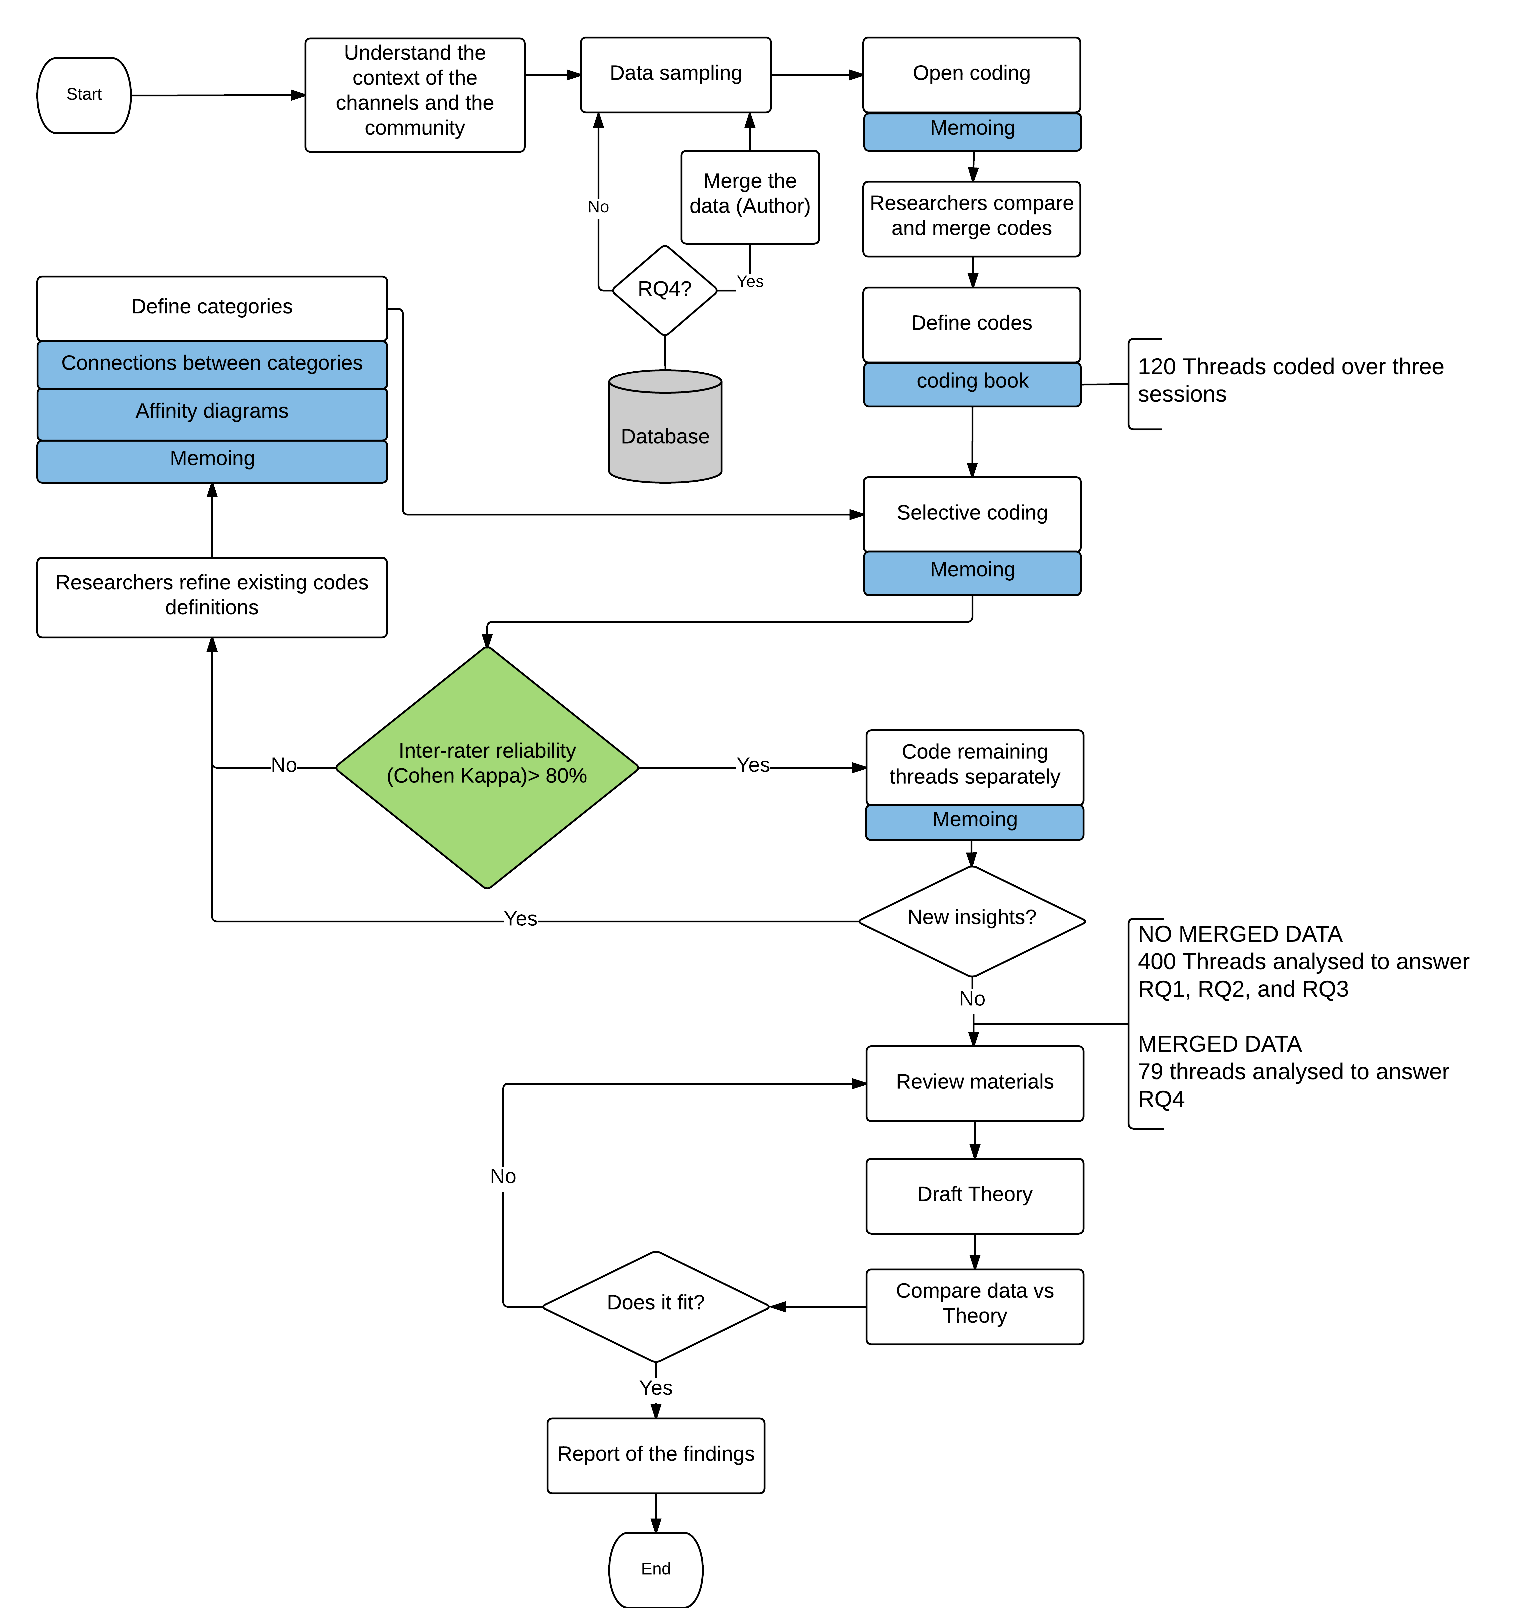
\includegraphics[width=\columnwidth]{Figures/ContentAnalysisFlow_3}
%		\caption[Our content analysis method]{Qualitative approach used to analyse Stack Overflow and the R-help mailing list data. The chart shows the process and techniques (coloured figures) used to analyse and develop the findings.}
%		\label{fig:ContentAnalysisFlow}
%	\end{figure}
%	%>>

%Figure \ref{fig:ContentAnalysisFlow} depicts a visual explanation of the data analysis process for this study.
%The coloured shapes depict the techniques used to support the data analysis, which are explained as follow:

The techniques used to support the data analysis, which are explained as follow:

	\begin{description}[itemsep=3pt, topsep=2pt, leftmargin=3em, parsep=0pt]
		\item[Memoing] is the act of taking notes (coding) on what the researcher is learning from the data during the analysis~\cite{Groenewald2008}.% for example, the hypotheses regarding a code, and relationships between concepts.
We wrote reflective memos in a spreadsheet next to the applicable codes (see figure \ref{fig:CodingExample}).
These memos were used to create the codes, and hypotheses about the relationships between concepts.

		\item[Affinity diagrams] allows to organize ideas and data into groups, and to find the relationships between concepts~\cite{Scupin1997}.
		We used them to discuss new insights, and while defining categories and relationships between them.

		\item[Inter-rater agreement \textit{Cohen Kappa}] is a coefficient used to measure the agreement between two coders who classify items into mutually exclusive categories~\cite{Stemler2004}.
		Ladis and Koch suggest that values above 0.60 or 60\% to obtain substantial results~\cite{Landis1977}.
		In a previous study~\cite{Gomez2013}, we used the same coefficient to measure agreement between coders.
		Based on this experience, we set a value above 0.80 or 80\% as the minimum to obtain substantial results.
		We used this coefficient after each coding session as a way to trigger discussion.

		\item[Code book] is a book that contains the definitions of the codes that researchers look during the data analysis~\cite{MacQueen1998}.
%		Codes are the building blocks for theory and foundations on which the researcher's argument rest.
%		We coded an initial set of 120 threads over three sessions.
%		In each session, we separately coded 40 threads.
		We coded in multiple sessions, which allowed us to refine the definitions.
		Each entry is associated with a title, a formal definition, an example, and space for notes from the researcher.
		The final version of the code book is detailed in section~\ref{cha:findings}.
	\end{description}

%\paragraph{The Analysis Process}

	The focus of the analysis is to \textit{understand the context of the media channels and the community}.
	The process consisted of:
	First, a recollection of the official information for both channels and the community to build a background of the community of practice and the channels studied.
%    From the channels, I collected posting guides, rules, channel objectives, and competitors, whereas from the community I collected the number of members, how it works, and the media channels that the community uses.
	Second, a mapping between messages from Stack Overflow with messages on the R-help mailing list.
    This is to overcome how the data is structured in both channels.
%    Stack Overflow has a clear delimitation of what is a question, an answer, a comment, a flag and an update, while the R-help mailing list is just plain text.
    The mapping of messages between both channels was as follows:

	\begin{description}[itemsep=3pt, topsep=2pt, leftmargin=3em, parsep=0pt]
		\item[Question:] the message is the first on the thread, and it contains the main question.
		\item[Answer:] the message provides a solution to the main question of the thread.
	 	\item[Update:] the message claims for a modification to a question (or answer) made by the author of such a question (or answer).
		\item[Comment:] the message offers a clarification to a specific part of the question or answer.
		\item[Flag:] the message requests attention from the moderator (e.g., repeated questions, spam, or rude behaviour).
	\end{description}

	To answer RQ1 and RQ2, we queried the database by selecting a random number of threads of each channels within a time frame.
	%<<
	The data set was capped at 400 threads for each channel when we deemed our observations as being saturated.
	To answer RQ3, we added a condition that matched, on both channels, messages with the same subject written by the same author.
	%>>
	The results were 79 threads, and therefore, we analysed the entire population available. 

%	To code the data, we used an \textit{open coding} technique that involves reporting \textit{what the researcher saw} during each coding session. 
%	The researcher has to keep in mind, all the time, the objective of the study and perform the coding based on it.
%	Each researcher coded the data on a separated way.
%	During the coding session, we wrote memos as needed, and marked repetitive patterns.
%	Later, we met to compare and discuss findings, and begin developing codes.

%	From our initial codes, we began the process of creating a \textit{coding book} to outline definitions. 
%	This set of codes were used later during the \textit{selective coding} step.
%	At this point, the researcher stops coding every occurrence, and begins seeing larger trends and connections within the data and codes.
%	It is possible that during the \textit{selective coding} step some codes have to be reformulated, or maybe split into more codes. 
%	Also, it is possible to formulate completely new codes as needed.
%	Whenever there is a new code or any is changed, it is necessary to go back and recode the material.

%	As a coding tool, my colleague and I used a spreadsheet in which each row represents a message of the thread.
%	%<<
%	If for any reason a message appeared to fit in more than one category, each researcher selected, at their own discretion, a primary category to represent the message.
%	%>>
%	Figure~\ref{fig:CodingExample} depicts an example of the coding spreadsheet that we used.
%	The number in the first column identifies if the message is a question, an answer or a comment. 
%	For instance, if the number assigned to the question was ``1'', then the answers were enumerated with consecutive numbers separated by a point (e.g., 1.1); and the comments were enumerated in a similar way to enumerated answers, but using three numbers: the first number represents the question, the second represents the answer, and the third represents the comment consecutive (e.g., 1.0.1). 
%	The second column contains the message, the third column the channel, the fourth column the question categorization, and so on.
%	The last column contains the URL to the thread on the channel.
%	Inside each cell, a semicolon ($;$) represents a sub-category, and the double pipe ($||$) divides two different ideas (e.g., in the \textit{MEMOS} column), or indicates that a message was re-classified after an update (e.g, \textit{ANSWER} column).

%	At the beginning of the coding, before we created the code book, the spreadsheet had only the \textit{ID}, the \textit{MESSAGE}, the \textit{MEMOS}, and the \textit{URL} columns.
%	During each iteration, the spreadsheet was updated with the classification and type of messages that my colleague and I were defining.

%	Originally, both researchers read the threads directly from the spreadsheet.
%	However, this method of reading turned out uncomfortable, and we fell back to read the threads directly from each channel rather than the spreadsheet.


\subsection{Phase 2: The survey} 

In \textit{phase 2}, we conducted a survey\footnote{A copy of the survey is available at \url{http://goo.gl/mxmH5J}} with members of the R community with the purpose of obtaining additional insights on the findings.
To test and refine the questions, format and tone, we performed two pilots.
%	First, I created a draft of the survey and did two pilots:
%	(1) with colleagues in our research group, and
%	(2) with R users at the University of Victoria.
%	The objective was to test and refine the questions, tone, rankings, and the format of the survey.
%	The survey questions were structured into five sections:
%	(1) the user,
%	(2) Stack Overflow use,
%	(3) the R-help mailing list use,
%	(4) Stack Overflow and the R-help mailing list if both used, and
%	(5) resources linked to used.
%	Survey's sections 2, 3 and 4 would only become active if the participant was a user of the channel.

We announced our survey on Twitter, Reddit, the R-help mailing list, and Meta Stack Exchange to reach users of both channels, and minimize the selection bias.
However, on Stack Exchange the announcement was not well received and therefore was deleted a few minutes later after posting it.
We received 26 valid responses out of 32 from the R community members.
%The survey did not collect any personal information.

%%% Local Variables:
%%% mode: latex
%%% TeX-master: "knowledge-curation.tex"
%%% End:
